%--- Header ------------------------------------------------------------

\documentclass[12pt]{article}
\usepackage{draft}
%\usepackage[onehalfspacing]{setspace}

\graphicspath{ {fig/} }
\hyphenation{}

%--- Meta data ---------------------------------------------------------

\usepackage{hyperref}
\hypersetup{
  pdfauthor   ={Jonas Schöley},
  pdftitle    ={},
  pdfsubject  ={},
  pdfkeywords ={},
  hidelinks,
  breaklinks=true,
  colorlinks=false
}

%--- Titlepage ---------------------------------------------------------

\begin{document}

%\begin{titlepage}

{\textbf{Title:}
Methods protocol for counterfactual life table analysis of excess mortality
\par\medskip}

{\textbf{Authors:}
Jonas Schöley$^{1}$
\par\medskip}

{\textbf{Affiliations:}\par
$^1$ Max Planck Institute for Demographic Research; Rostock, Germany\par
\par\medskip}

\tableofcontents

%\end{titlepage}

%--- Text --------------------------------------------------------------

\section{Summary}

We calculate life tables and associated life expectancies by sex for a selection of 34 countries for the years 2000 through 2024. For the years 2020 through 2024 we calculate counterfactual life expectancies based on the continuation of pre-pandemic mortality trends and derive associated life expectancy deficits -- the difference between actual and counterfactual life expectancy -- as an age standardized and trend adjusted measure of excess mortality.

The data basis for our calculation are midyear population and death counts by age, sex, and country sourced from the Short Term Mortality Fluctuations Database (HMD-STMF \cite{jdanov2021b}), the Human Mortality Database (HMD, \cite{HMD2025, Barbieri2015}), the UN World Population Prospects (WPP-2024 \cite{UnitedNationsDepartmentforEconomicandSocialAffairs2025}), and national statistical offices (ONS \cite{officefornationalstatistics2025}, CDC \cite{centersfordiseasecontrolandprevention2025}). For a complete list of sources by country see methods appendix ``Data sources''.

Age specific death counts are harmonized to a single year age grouping with open age group 100+ using the PCLM method \citep{Rizzi2015, Pascariu2018}. Weekly death counts are aggregated to annual counts and midyear population estimates are converted to person years of exposure adjusting for the effect of leap weeks. To adjust for systematic bias in registered deaths between annualized STMF data and HMD annual totals we estimate correction factors based on a statistical model (see methods appendix ``Bias correction of age specific annual death counts'').

Given the harmonized annual death counts and population exposures by age and sex we calculate period life tables using the standard piecewise-exponential model. We then fit a Poisson-Lee-Carter model \citep{Lee1992} using the R library \texttt{StMoMo} \citep{Villegas2015} to the available pre-pandemic data since 2000 and forecast counterfactual age specific mortality rates and death counts over the years 2020 through 2024. Life expectancy deficits (LED) are then derived along with P-scores \citep{Ullrich-Kniffka2024} and the Mean unfulfilled lifespan (MUL, \cite{Heuveline2021}) as alternative measures of excess. We decompose the life expectancy deficits into age specific contributions using the Arriaga method \citep{Arriaga1984}.

Throughout the analysis population exposures and annual death counts by sex are aggregated as needed to derive results for both sexes combined and for the joint period 2020-2024.

We perform simulation based uncertainty propagation throughout our analysis via a Poisson parametric bootstrap of the life table estimates and a random walk simulation of the Lee-Carter forecast. Based on this we derive a p-value for the estimated life expectancy deficit, i.e. the probability of observing or exceeding an estimated life expectancy deficit given the continuation of pre-pandemic trends.

The complete analysis workflow is explained in detail in the methods appendix. The analysis script is available from \href{https://github.com/jschoeley/e0deficit}{\texttt{https://github.com/jschoeley/e0deficit}}.

\section{Data}

\subsection{Data sources}

The basis for our analysis are death and population counts by age, year, sex, and country. We source\footnote{
\href{https://github.com/jschoeley/e0deficit/blob/main/src/12-download_death.R}{\texttt{github.com/jschoeley/e0deficit/blob/main/src/12-download\_death.R}}
\href{https://github.com/jschoeley/e0deficit/blob/main/src/11-download_population_and_rates.R}{\texttt{github.com/jschoeley/e0deficit/blob/main/src/11-download\_population\_and\_rates.R}}
} the death counts from:

\begin{itemize}
    \item The Human Mortality Database (HMD, \cite{HMD2025, Barbieri2015}) for annual death counts and exposures by age and sex for those countries for which a complete series is available through 2024.
    \item The Short-term mortality fluctuations (HMD-STMF, \cite{jdanov2021b}) input data base for weekly death counts by age and sex across countries. The data is updated weekly and includes the most recent information on death counts. We derive annual counts from this source in cases where the HMD does not provide data through 2024.
    \item The UK's Office for National Statistics (ONS, \cite{officefornationalstatistics2025}) annual death counts by age and sex for England and Wales. We use this data for years 2010 through 2019 because the age grouping in the HMD-STMF data for these years is too coarse for reliable life expectancy estimates.
    \item The US Centers for Disease Control and Prevention (CDC, \cite{centersfordiseasecontrolandprevention2025}) for annual death counts by age and sex for the United States. We use this data for years 2000 through 2019 for the US, lacking any HMD-STMF data for these years.
\end{itemize}

Population data form the basis for our person year exposure estimates and are sourced from:

\begin{itemize}
    \item The World Population Prospects 2024 (WPP-2024, \cite{UnitedNationsDepartmentforEconomicandSocialAffairs2025}) for midyear population estimates and projections by age, year and country.
    \item The HMD for midyear population estimates by age, year and country for those countries for which a complete series is available through 2024 and for the regions of the UK.
\end{itemize}

%Furthermore, in order to perform the population projections, we source:
%
%\begin{itemize}
%    \item Age specific fertility rates by country and year from WPP-2024.
%    \item Age specific fertility rates by country and year from the HFD for all HMD/HFD regions
%    \item Age specific migration projections by country and year from Eurostat.
%    \item Age specific death rates by country, sex, and year from HMD
%\end{itemize}

For a list of data sources by country and year see Table \ref{tab:sources}.

\renewcommand{\arraystretch}{0.9}
\begin{table}[ht!]
\footnotesize
\begin{tabular*}{\linewidth}{@{\extracolsep{\fill}}llll}
\toprule
Country & Period & Death counts & Population \\ 
\midrule\addlinespace[2.5pt]
Austria & 2000-2024 & HMD-STMF & WPP-2024 \\ 
Belgium & 2000-2024 & HMD & HMD-EST \\ 
Bulgaria & 2000-2024 & HMD-STMF & WPP-2024 \\ 
Switzerland & 2000-2024 & HMD & HMD-EST \\ 
Chile & 2000-2015 & HMD & WPP-2024 \\ 
Chile & 2016-2024 & HMD-STMF & WPP-2024 \\ 
Czech Republic & 2000-2004 & - & WPP-2024 \\ 
Czech Republic & 2005-2024 & HMD-STMF & WPP-2024 \\ 
Germany & 2000-2024 & HMD-STMF & WPP-2024 \\ 
Denmark & 2000-2024 & HMD & HMD-EST \\ 
Estonia & 2000-2024 & HMD & HMD-EST \\ 
Spain & 2000-2024 & HMD-STMF & WPP-2024 \\ 
Finland & 2000-2024 & HMD & HMD-EST \\ 
France & 2000-2024 & HMD-STMF & WPP-2024 \\ 
England and Wales & 2000-2009 & - & HMD-EST \\ 
England and Wales & 2010-2019 & ONS & HMD-EST \\ 
England and Wales & 2020-2022 & HMD-STMF & HMD-EST \\ 
England and Wales & 2023-2024 & HMD-STMF & HMD-PRJ \\ 
Northern Ireland & 2000-2021 & HMD & HMD-EST \\ 
Northern Ireland & 2022 & HMD-STMF & HMD-EST \\ 
Northern Ireland & 2023-2024 & HMD-STMF & HMD-PRJ \\ 
Scotland & 2000-2022 & HMD-STMF & HMD-EST \\ 
Scotland & 2023-2024 & HMD-STMF & HMD-PRJ \\ 
Greece & 2000-2014 & HMD & WPP-2024 \\ 
Greece & 2015-2024 & HMD-STMF & WPP-2024 \\ 
Croatia & 2000 & - & WPP-2024 \\ 
Croatia & 2001-2024 & HMD-STMF & WPP-2024 \\ 
Hungary & 2000-2024 & HMD-STMF & WPP-2024 \\ 
Israel & 2000-2024 & HMD-STMF & WPP-2024 \\ 
Iceland & 2000-2024 & HMD-STMF & WPP-2024 \\ 
Italy & 2000-2010 & - & WPP-2024 \\ 
Italy & 2011-2024 & HMD-STMF & WPP-2024 \\ 
Japan & 2000-2024 & HMD & HMD-EST \\ 
Lithuania & 2000-2024 & HMD & HMD-EST \\ 
Luxembourg & 2000-2024 & HMD-STMF & WPP-2024 \\ 
Latvia & 2000-2024 & HMD & HMD-EST \\ 
Netherlands & 2000-2024 & HMD-STMF & WPP-2024 \\ 
Norway & 2000-2024 & HMD & HMD-EST \\ 
Poland & 2000-2024 & HMD-STMF & WPP-2024 \\ 
Portugal & 2000-2024 & HMD & HMD-EST \\ 
Sweden & 2000-2024 & HMD & HMD-EST \\ 
Slovenia & 2000-2024 & HMD-STMF & WPP-2024 \\ 
Slovakia & 2000-2024 & HMD & HMD-EST \\ 
Taiwan & 2000-2024 & HMD-STMF & WPP-2024 \\ 
USA & 2000-2019 & CDC & WPP-2024 \\ 
USA & 2020-2024 & HMD-STMF & WPP-2024 \\ 
\bottomrule
\end{tabular*}
\caption{Data sources by country and year.}
\label{tab:sources}
\end{table}

\subsection{Data harmonization}

\subsubsection{Death count age harmonization}

As the HMD-STMF input data is not harmonized in terms of age grouping we perform\footnote{\href{https://github.com/jschoeley/e0deficit/blob/main/src/21-harmonize_death_with_exposures.R}{\texttt{https://github.com/jschoeley/e0deficit/blob/main/src/21-harmonize\_death\_with\_exposures.R}}} a model based ungrouping of deaths into single ages for each region-year-sex stratum using the Penalized Composite Link Method (PCLM) \citep{Rizzi2015} implemented in the R package \texttt{ungroup} \citep{Pascariu2018}.

The original death counts over single year age groups $\mathbf{d}^\mathrm{single}=\left(d_{j=1}, \ldots, d_J\right)^\intercal$ have been grouped (summed) into discrete age bins $\mathbf{d}^\mathrm{grouped}=\left(d_{i=1}, \ldots, d_I\right)^\intercal$ of varying width. We assume the grouped death counts to arise from a Poisson distribution with mean $\mu_i$:

$$
d^\mathrm{grouped}_i \sim \mathrm{Poisson}\left(\mu_i\right).
$$

The PCLM methods seeks to recover the means of the original single year death counts, $\boldsymbol{\gamma} = \left(\gamma_{j=1}, \ldots, \gamma_J\right)^\intercal$. To that end, one can encode the age aggregation into a binary composition matrix $\mathbf{C}$ with dimensions $I\times J$ such that $\mathbf{d}^\mathrm{grouped} = \mathbf{C}\mathbf{d}^\mathrm{single}$. The grouped Poisson rates are then connected to the single age means via the composite link

$$
\boldsymbol{\mu} = \mathbf{C}\boldsymbol{\gamma}.
$$

By specifying that the $\boldsymbol{\gamma}$ are a smooth function of age,

$$
\gamma_j = \exp\left(s(x(j)\right),
$$

where $s(x(j))$ is a P-spline over the starting age $x$ of single year age groups $j \in 1,\ldots,J$, a penalized likelihood solution can be found for the vector of mean death counts by single age. To get an integer estimate of the death count in single age $x$ we round $\gamma_x(j)$ down to the next integer,

$$
\hat{d_x}^\mathrm{single} = \lfloor\gamma_{x(j)}\rfloor,
$$

such that $\hat{d_x}$ corresponds to the mode of the Poisson distribution with rate $\gamma_{x(j)}$.

Because the age grouping scheme may vary within a year, the ungrouping is separately applied to each region $\times$ sex $\times$ year $\times$ age pattern combination in the input data. In a final step, the harmonized sub-annual HMD-STMF death counts are summed into annual death counts by age, $\hat{d}_{xy}$.

\subsubsection{Exposure time calculation}

We derive person years of exposure by age and year, $E_{xy}$, from the midyear population estimates, $N_{xy}^\mathrm{midyear}$. We choose the HMD midyear population for exposure calculation for those countries where a complete series is available through 2024 and for the regions of UK. Otherwise we choose the World Population Prospects 2024 data which is always complete throughout 2024. To complete HMD exposures for the UK regions we perform a stable population projection based on the most recent HMD population data and 5 year average (2015 through 2019) age specific mortality and fertility rates. Exposures are adjusted for the length of the observation period within a year, taking into account weeks with missing data and leap-weeks.

$$
E_{xy} = N_{xy}^\mathrm{midyear}n_y^\mathrm{observed-weeks}/52.
$$

\subsubsection{Bias correction of age specific annual death counts}

The purpose of our bias correction model is to correct any systematic deviations between our age specific mortality rate estimates and the official annual estimates. While the HMD-STMF death counts allow for timely estimates of current mortality they sometimes deviate substantially from official annual estimates due to different population definitions and reporting guidelines in the weekly death reporting compared to the annual reporting. Because these systematic biases are stable in time, they can be estimated and corrected. To that end we estimate\footnote{\href{https://github.com/jschoeley/e0deficit/blob/main/src/31-rate_bias_correction.R}{\texttt{https://github.com/jschoeley/e0deficit/blob/main/src/31-rate\_bias\_correction.R}}} a correction factor $\widehat{c}_{xy}$ which, if multiplied with the single age annual death counts, $\widehat{d}_{xy}$, yields the corrected counts:

\begin{equation*}
  \widehat{d}_{xy}^\mathrm{corrected} = \widehat{c}_{xy}\cdot\widehat{d}_{xy}.
\end{equation*}

We estimate the correction factor via the Poisson model

$$
d_{xy}^\mathrm{benchmark} \sim \mathrm{Poisson}\left(c_{xy}\cdot\widehat{d}_{xy}\right),
$$

where the benchmark death counts are taken from the HMD and

$$
c_{xy} = \exp(s_{y}(x|y)),
$$

is a smooth age effect estimated separately for each year capturing the time varying deviations between uncorrected and benchmark death counts. The correction factor from the last year with available benchmark data will be used in subsequent years.

Figures \ref{fig:biascorrection-a} and \ref{fig:biascorrection-b} show the estimated correction factors and the bias corrected age specific death counts by year for the example of Austrian females. The model is fit separately to each region and sex.

\begin{figure}
    \centering
    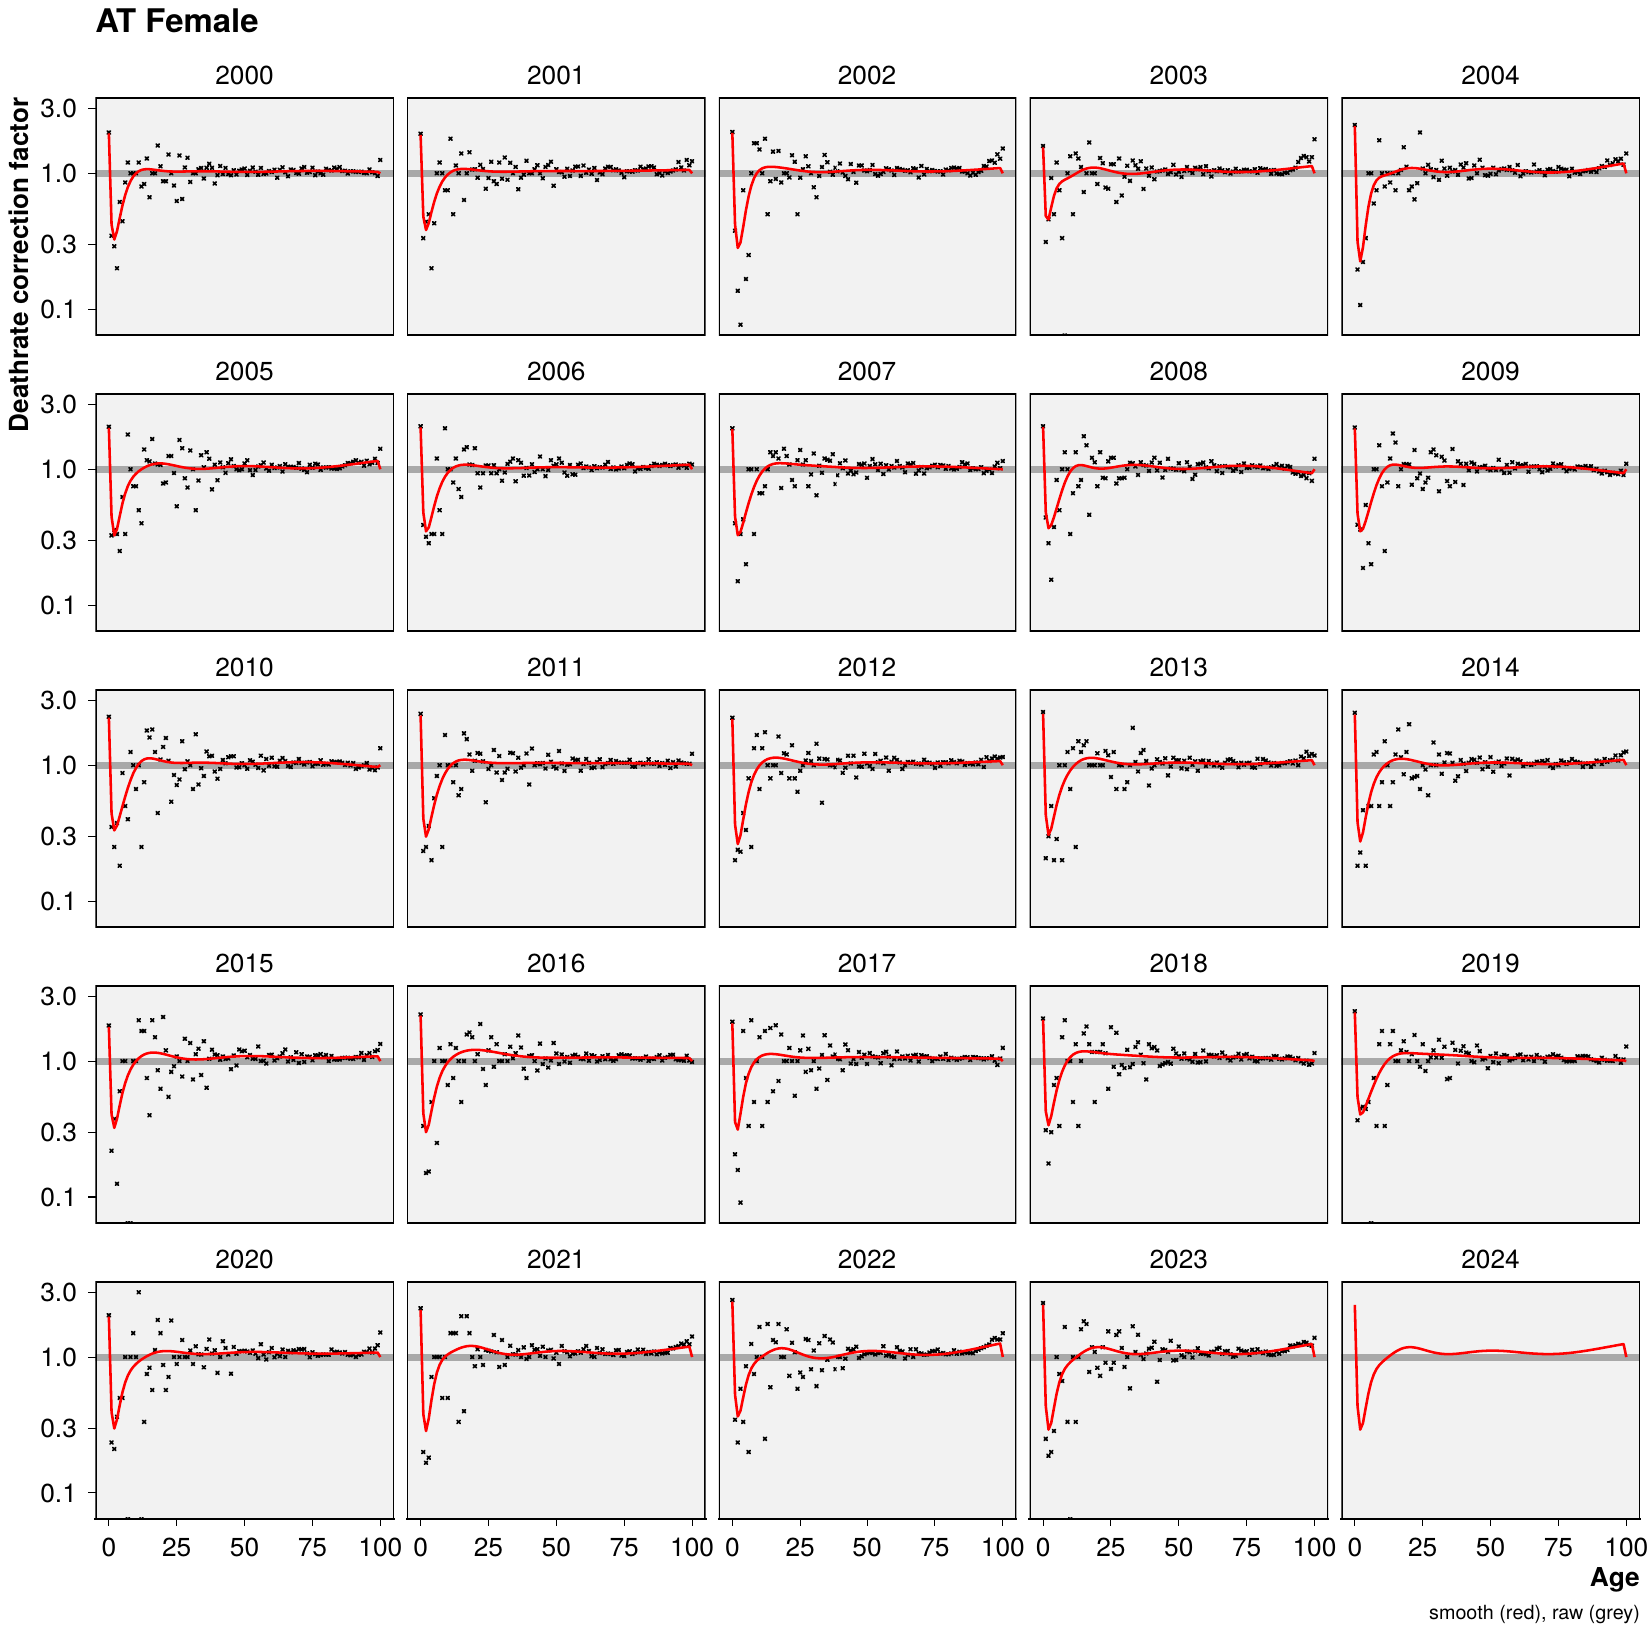
\includegraphics{31-bias_correction_diagnostics_b.png}
    \caption{Demonstration of estimated (red) bias correction factors $c_{xy}$ vs. raw correction factors (black) for Austrian females.}
    \label{fig:biascorrection-a}
\end{figure}


\begin{figure}
    \centering
    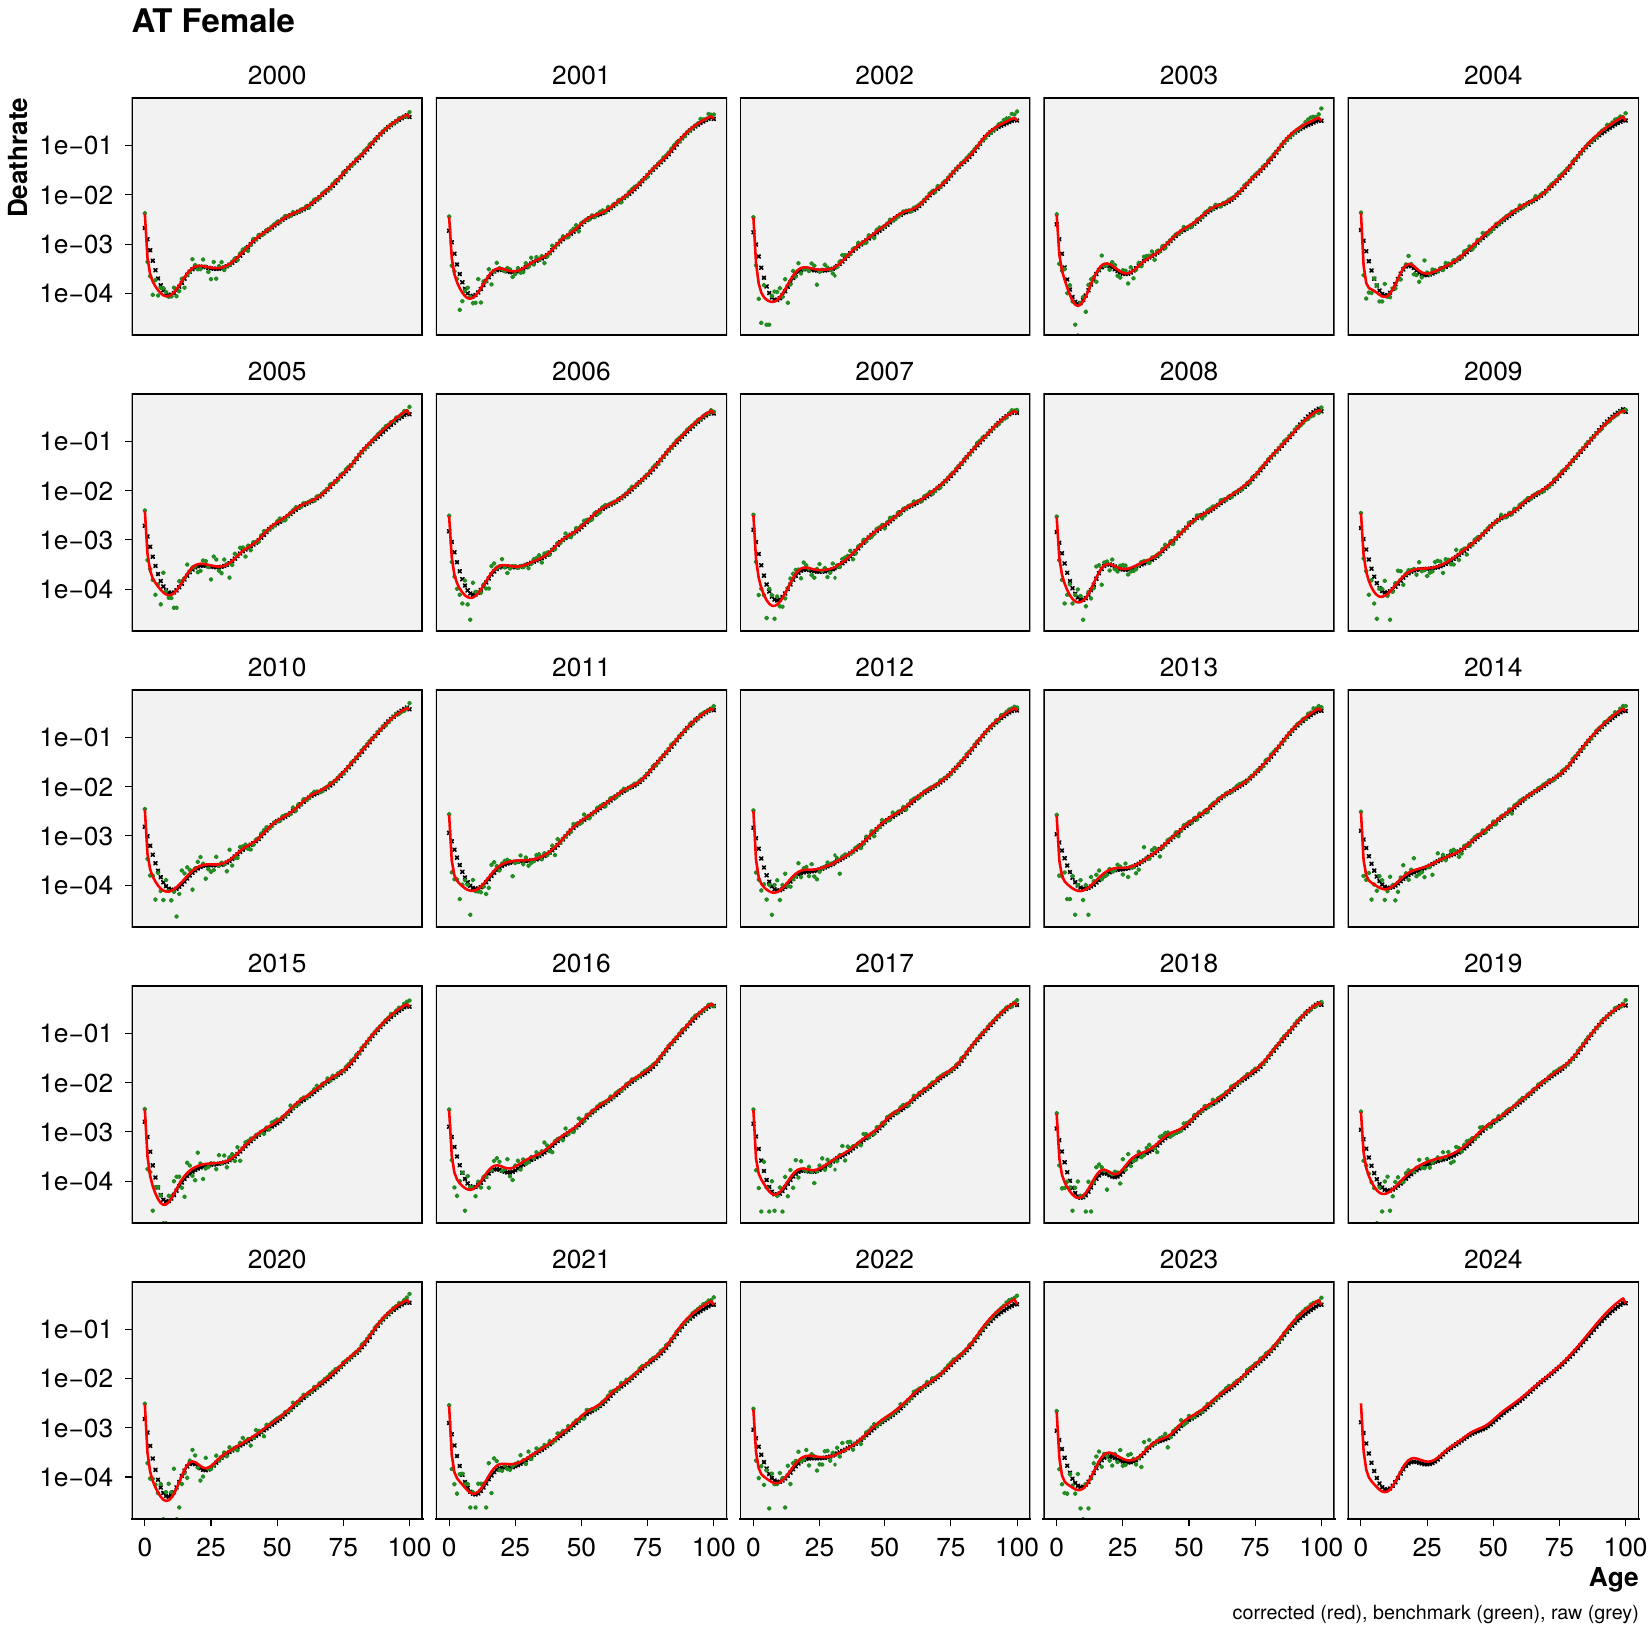
\includegraphics{31-bias_correction_diagnostics_a.png}
    \caption{Demonstration of bias corrected ungrouped age specific death rates (red) vs. non-corrected death rates (black) and HMD benchmark death rates (green) for Austrian females.}
    \label{fig:biascorrection-b}
\end{figure}

\section{Analysis}

\subsection{Counterfactual mortality forecast}

In order to calculate the life expectancy under continuation of pre-pandemic trends we forecast\footnote{\href{https://github.com/jschoeley/e0deficit/blob/main/src/40-counterfactual_projection.R}{\texttt{https://github.com/jschoeley/e0deficit/blob/main/src/40-counterfactual\_projection.R}}} age specific mortality rates over the years 2020-2024 using a Poisson-Lee-Carter model given the data available up to January 2020.

We fit a Poisson-Lee-Carter model \citep{Lee1992} where death counts at single age $x$ and single year $y$ are distributed

$$
d_{xy} \sim \mathrm{Poisson}(\mu_{xy}~E_{xy}),
$$

with death rates

$$
\mu_{xy}=\exp(\alpha_x + \beta_x\kappa_y),
$$

and identifiability constraints $\sum_y \kappa_y=0$ and $\sum_x \beta_x = 1$.

We forecast $\mu_{xy}$ past the fitting period via the usual random walk with drift over $\kappa_y$,

$$
\kappa_{y+1} = \kappa_y + \widehat{b} + \mathrm{Normal(0, \widehat{\sigma})}.
$$

We estimate the variance and mean difference of the estimated year-on-year $\kappa_y$ changes and simulate a corresponding random walk with drift over the years 2020-2024. The resulting forecasts of $\kappa$ are then used to derive a corresponding surface of age-period mortality rates $\mu^\mathrm{expected}_{xy}=\exp\left(\alpha_x + \beta_x\kappa_y\right)$ for forecast horizon $y \in \{2020, 2021, \ldots, 2024\}$. We fit the model using the R library \texttt{StMoMo} \citep{Villegas2015}. Forecast uncertainty is propagated throughout the rest of the analysis via 250 samples of the forecasted $\mu^\mathrm{expected}_{xy}$.

\subsection{Life table inference}

We perform a parametric bootstrap of our life table estimates\footnote{\href{https://github.com/jschoeley/e0deficit/blob/main/src/50-estimation_and_inference.R}{\texttt{https://github.com/jschoeley/e0deficit/blob/main/src/50-estimation\_and\_inference.R}}} based on 250 Poisson replicates of actual and expected age specific death counts for any population under consideration (for brevity sex, country, and year indices are omitted in this section).

$$
  d_{x}^\mathrm{actual} \sim \mathrm{Poisson}\left( \widehat{d}_{x}^\mathrm{corrected} \right) \\
$$

$$
  d_{x}^\mathrm{expected} \sim \mathrm{Poisson}\left( \mu^\mathrm{expected}\cdot E_{x} \right)
$$

At this point we aggregate the simulated death counts along with the person years of exposure into larger populations of interest, e.g. male and female are summed to total population and annual data are summed to multi-year aggregates. All of the following analysis steps are also performed for the newly created aggregated populations.

For any given population and for each sample draw we calculate the actual and expected central death rates by age as

$$
  m_{x}^\mathrm{actual} = d_{x}^\mathrm{actual} / E_{x},
$$

and

$$
  m_{x}^\mathrm{expected} = d_{x}^\mathrm{expected} / E_{x}.
$$

These rates are then transformed into life tables yielding actual and expected life expectancies, $e_{x}^\mathrm{actual}$ and $e_{x}^\mathrm{expected}$, for each population, year, and simulation draw. We write $n_x = 1$ for $x \neq \omega$ and $n_\omega = \infty$ for the width of the age group starting at $x$ with $\omega = 100$ being the open age group closing the life table. Under the piecewise constant assumption we calculate the life tables as

\begin{align*}
  \Pr(X \geq x+n|X>x) = {}_np_{x} &= \begin{cases}
    0 & \mathrm{if}~x = \omega \\
    \exp(-{}_nm_{x}n_x) & \mathrm{otherwise}
  \end{cases} \\
  \Pr(X>x) = \ell_{x} &= \begin{cases}
    1 & \mathrm{if}~x = 0\\
    \prod_{i=0}^{x-1} {}_np_{x=i} & \mathrm{otherwise}
  \end{cases} \\
  \Pr(x\leq X < x+n) = {}_nd_{x} &= \begin{cases}
    \ell_\omega & \mathrm{if}~x = \omega \\
    \ell_{x+n}-\ell_{x} & \mathrm{otherwise}
  \end{cases} \\
  \int_x^{x+n}\ell_a\,\mathrm{d}a = {}_nL_{x} &= \begin{cases}
    1/{}_nm_x & \mathrm{if}~x = \omega \\
    {}_nd_{x}/{}_nm_{x} & \mathrm{otherwise}
  \end{cases} \\
  \int_x^{\infty}\ell_a\,\mathrm{d}a = T_{x} &= \sum_{i=x}^\omega {}_nL_{x=i} \\
  \mathbb{E}(X|X>x) = e_x &= T_x/\ell_x.
\end{align*}

Now the \emph{life expectancy deficit} can be calculated as the difference between actual and counterfactual life expectancy, the baseline life expectancy under the continuation of pre-pandemic trends,

$$
e_{0}^\mathrm{deficit} = e_{0}^\mathrm{actual} - e_{0}^\mathrm{expected}.
$$

Note that we define the deficit such that it is negative if actual life expectancy falls short of the expectation, i.e. if there are excess deaths, and positive if there is a life expectancy surplus, i.e. if the expectation is outperformed.

Life expectancy deficits do not necessarily indicate a structural deviation from expected mortality trends as both the expected and the observed life tables are subject to uncertainty. Uncertainty in the expectation is mainly due to forecasting error -- we do not know exactly how age specific mortality rates would have developed in the absence of the pandemic. This uncertainty is captured by the random walk of the forecasting model described earlier. Additionally, aleatoric uncertainty in the death counts induces uncertainty in the estimated central death rates which is reflected via our Poisson re-sampling scheme.

Due to the stated sources of randomness one may observe life expectancy deficits even under the continuation of pre-pandemic trends. Thus we perform inference about the estimated $e_{0}^\mathrm{deficit}$ by calculating a p-value stating the probability of estimating a life expectancy deficit as large as the realized deficit under the continuation of pre-pandemic trends.  Life expectancy deficits under the null hypothesis of pre-pandemic trends are defined as

$$
  T = e_{0}^\mathrm{expected}-\mathbb{E}\left(e_{0}^\mathrm{expected}\right),
$$

and we derive the sampling distribution of $T$ from our sample draws of $e_{0}^\mathrm{expected}$. We can then calculate the probability of our calculated $e_{0}^\mathrm{deficit}$ given pre-pandemic trends as

$$
  \Pr\left(e_{0}^\mathrm{deficit}\leq T^*\right).
$$

Figure \ref{fig:pval} demonstrates the procedure.

\begin{figure}
    \centering
    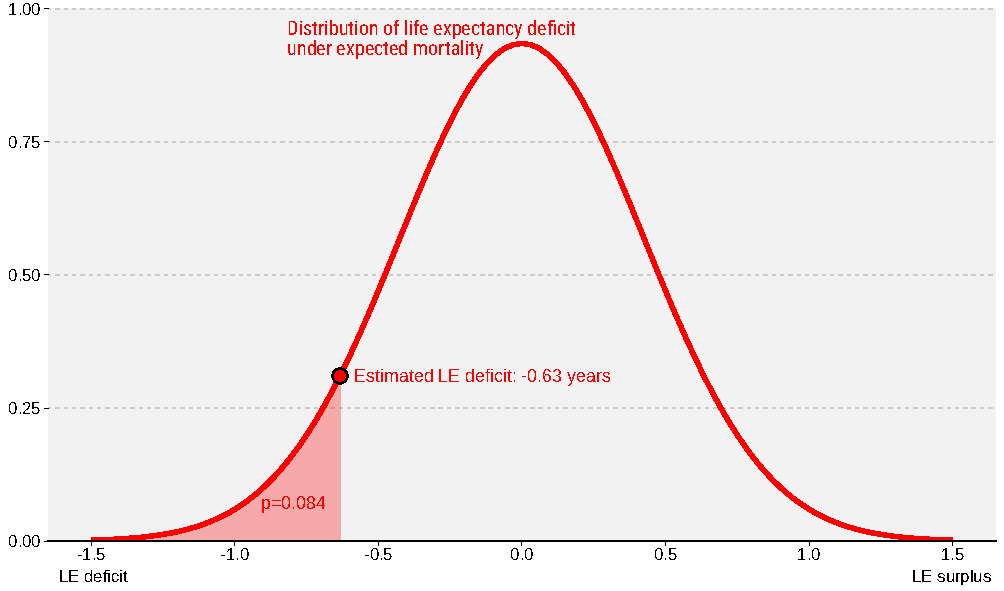
\includegraphics{50-pval.pdf}
    \caption{Demonstration of p-value calculation for estimated life expectancy deficit.}
    \label{fig:pval}
\end{figure}

\subsection{Clustering of life expectancy deficits}

We calculate time series of life expectancy deficits, $e_{0,y}^\mathrm{deficit}$, for years 2020 through 2024 by region. These series are then clustered\footnote{\href{https://github.com/jschoeley/e0deficit/blob/main/src/51-assign_clusters.R}{\texttt{https://github.com/jschoeley/e0deficit/blob/main/src/51-assign\_clusters.R}}} into four groups: A) Early peak (peak deficit in 2020 or 2021 without pronounced worsening in 2021), B) Second wave peak (pronounced peak deficit in 2021), C) Late peak (worsening of deficits starting 2022), and D) Prolonged depression (deficits since 2020 without pronounced peak or trend). To establish robustness, we compare the group assignment under three different clustering procedures.

\emph{Hierarchical clustering}

The group assignment for each country's deficit trajectory is formalized by employing hierarchical clustering with a pre-specified cluster number of four. We cluster on deficit series for both sexes combined. Prior to clustering we derive three time series features for each region $c$: the range of the deficits, $r_c = \max\limits_y(e_{0,y,c}^\mathrm{deficit}) - \min\limits_y(e_{0,y,c}^\mathrm{deficit})$, the centered and range normalized trajectory of deficits, $s_{y,c}=\left(e_{0,y,c}^\mathrm{deficit}-\underset{y}{\mathrm{mean}}(e_{0,y,c}^\mathrm{deficit})\right) / r_c$, and the first differences of $s_{y,c}$ over time. We then run the hierarchical clustering algorithm implemented in the R package \texttt{dtwclust} with Euclidean distance and Ward's minimum variance method on the combined vector of features across regions to determine each regions cluster. The resulting clustering captures the phenomenology of the four qualitative groups described above.

\emph{Probabilistic decision rule}

A similar cluster assignment can be achieved with a much simpler method of decision rules over our posterior simulation draws. First we test if a countries life expectancy deficit series features a significant ($\alpha = 0.1$) peak or slope. If no, we assign the group D, otherwise we check if the probability for 2021 being the peak deficit year is $\geq 90\%$. If yes, we assign the group B, otherwise we check if the mean peak deficit was later than 2021. If yes we assign group C, otherwise group A. This method achieves an overlap of 85.3\% in cluster assignment with the hierarchical clustering method.

\emph{Non-probabilistic decision rule}

An even simpler, entirely non-probabilistic, algorithm for cluster assignment can be defined by labeling as group D every country where the deficit peak is less than 0.2 years above the deficit in neighboring years and the range is less than 0.75 years. For all remaining countries the year of peak deficit determines group A (2020), group B (2021), or group C (later than 2021). This simplistic method assigns the same label as the hierarchical clustering method in 82.4\% of regions.

Table \ref{tab:cluster} shows the cluster assignments per country under the three different clustering procedures. The results in the paper are reported under the hierarchical clustering.

\begin{table}[h]
\begin{tabular}{lccc}
\toprule
Region & Hierarchical & Probabilistic & Non-probabilistic \\
\midrule
AT          & D            & D              & D              \\
BE          & A            & A              & A              \\
BG          & B            & B              & B              \\
CH          & A            & A              & A              \\
CL          & B            & B              & B              \\
CZ          & B            & B              & B              \\
DE          & D            & C              & C              \\
DK          & C            & C              & C              \\
EE          & B            & B              & B              \\
ES          & A            & A              & A              \\
FI          & C            & C              & C              \\
FR          & D            & C              & C              \\
GB-EAW      & A            & A              & A              \\
GB-NIR      & D            & C              & C              \\
GB-SCT      & A            & A              & B              \\
GR          & B            & B              & B              \\
HR          & B            & B              & B              \\
HU          & B            & B              & B              \\
IL          & D            & C              & C              \\
IS          & C            & C              & C              \\
IT          & A            & A              & A              \\
JP          & C            & C              & C              \\
LT          & B            & B              & B              \\
LU          & A            & D              & A              \\
LV          & B            & B              & B              \\
NL          & D            & D              & D              \\
NO          & C            & C              & C              \\
PL          & B            & B              & B              \\
PT          & D            & D              & D              \\
SE          & A            & A              & A              \\
SI          & A            & A              & B              \\
SK          & B            & B              & B              \\
TW          & C            & C              & C              \\
US          & B            & B              & B \\\bottomrule
\end{tabular}
\caption{\label{tab:cluster}Regional cluster assignments under different clustering procedures.}
\end{table}

\subsection{Age decomposition analysis}

We perform the Arriaga decomposition \citep{Arriaga1984} to attribute life expectancy deficits to age specific excess mortality\footnote{\href{https://github.com/jschoeley/e0deficit/blob/main/src/50-estimation_and_inference.R}{\texttt{https://github.com/jschoeley/e0deficit/blob/main/src/50-estimation\_and\_inference.R}}}. As the Arriaga decomposition is analytic and can be expressed as a series of simple arithmetic operations it lends itself well to simulation based inference where computation speed is vital. Based on the previously estimated life table quantities we calculate

\begin{align*}
  {}_n\mathrm{DE}_x &= \left({}_nL_{x}^\mathrm{actual} / \ell_{x}^\mathrm{actual} -
  {}_nL_{x}^\mathrm{expected} / \ell_{x}^\mathrm{expected}\right)\cdot \ell_{x}^\mathrm{actual} \\
  {}_n\mathrm{IE}_x &=
    \left(
      \ell_x^\mathrm{expected} / \ell_x^\mathrm{actual} -
      \ell_{x+n}^\mathrm{expected} / \ell_{x+n}^\mathrm{actual}
    \right) \cdot
    T_{x+n},
\end{align*}

which yields the contribution of excess mortality at age $x$ to the overall life expectancy deficit:

$$
{}_n\Delta_x^{e_0} = {}_n\mathrm{DE}_x + {}_n\mathrm{IE}_x.
$$

\section{Robustness and sensitivity}

\subsection{Benchmark tests}

\footnote{\href{https://github.com/jschoeley/e0deficit/blob/main/src/91-benchmark_check_e0.R}{\texttt{https://github.com/jschoeley/e0deficit/blob/main/src/91-benchmark\_check\_e0.R}}}

\begin{figure}
    \centering
    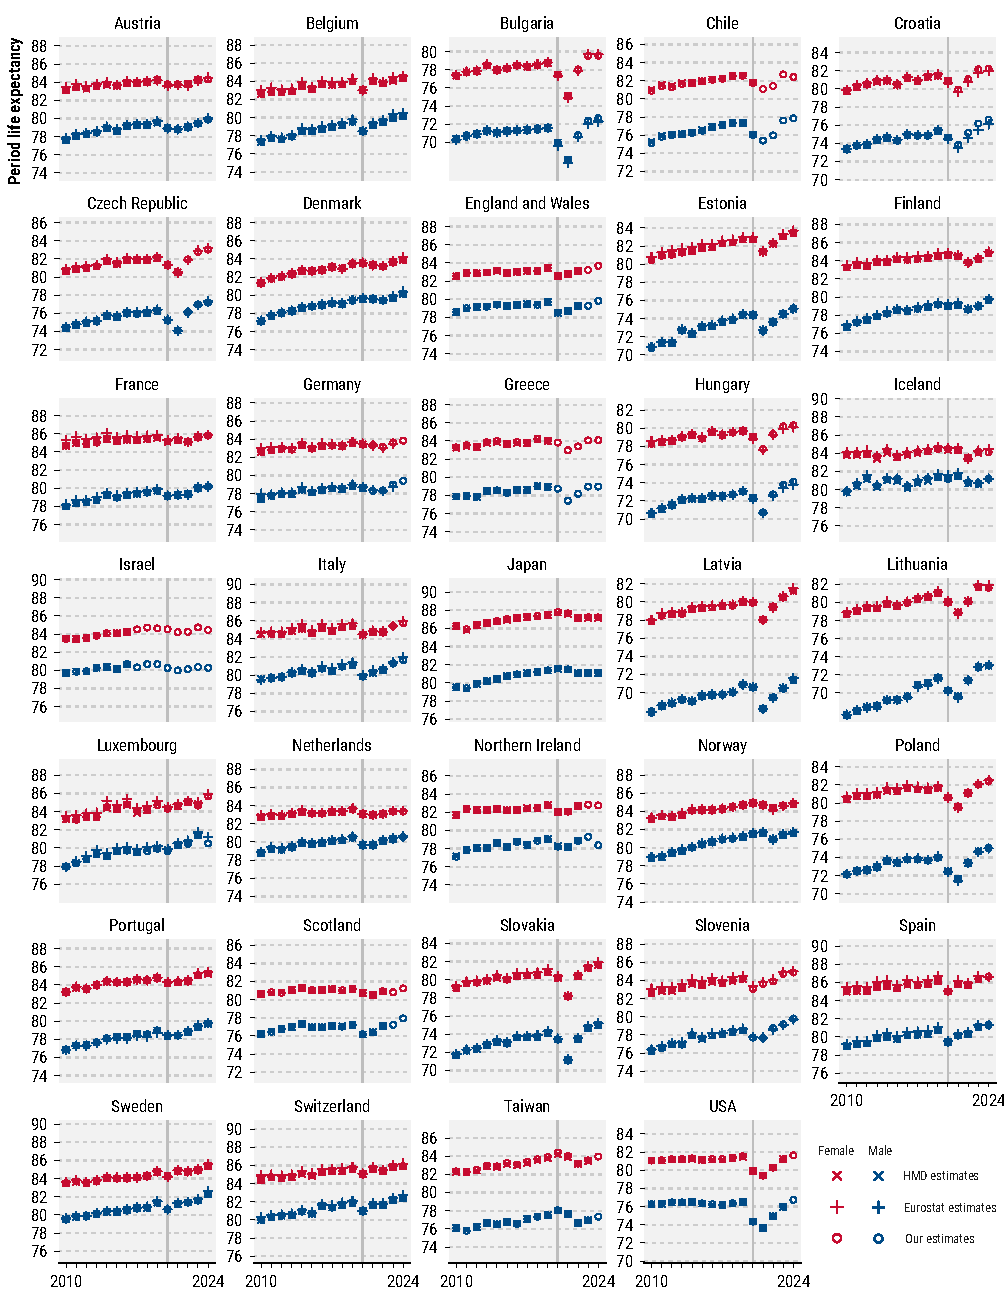
\includegraphics{91-e0benchmark.pdf}
    \caption{Comparison of our life expectancy estimates with past estimates by Eurostat and the Human Mortality Database.}
    \label{fig:benchmark}
\end{figure}

\clearpage

\subsection{Alternative measures of excess mortality}

\footnote{\href{https://github.com/jschoeley/e0deficit/blob/main/src/92-sensitivity_check_excess_measures.R}{\texttt{https://github.com/jschoeley/e0deficit/blob/main/src/92-sensitivity\_check\_excess\_measures.R}}}

In addition to the life expectancy deficit we calculate alternative measures of excess mortality as a sensitivity check.

Excess deaths are the difference between actual and expected deaths,

$$
\mathrm{Excess}_x = d_{x}^\mathrm{actual}-d_{x}^\mathrm{expected}
$$

and can be turned into the P-score\citep{Ullrich-Kniffka2024} by aggregating over age and expressing them as a ratio to total expected deaths,


$$
\mathrm{Pscore} = \sum_x \frac{\mathrm{Excess}_x}{d_{x}^\mathrm{expected}}.
$$

The mean unfulfilled lifespan (MUL, \citep{Heuveline2021}), like the life expectancy deficit, is based on counterfactual life expectancies. MUL is defined as the difference between the average age at death during some period and the average expected age at death under counterfactual mortality conditions.

$$
\mathrm{MUL} = \frac{1}{\sum_x d_{x}^\mathrm{actual}}\sum_x \mathrm{Excess}_x\cdot e_{x}^\mathrm{expected}.
$$

Figure \ref{fig:excessmeasures} shows a comparison of the three measures with each other actoss countries.

\begin{figure}
    \centering
    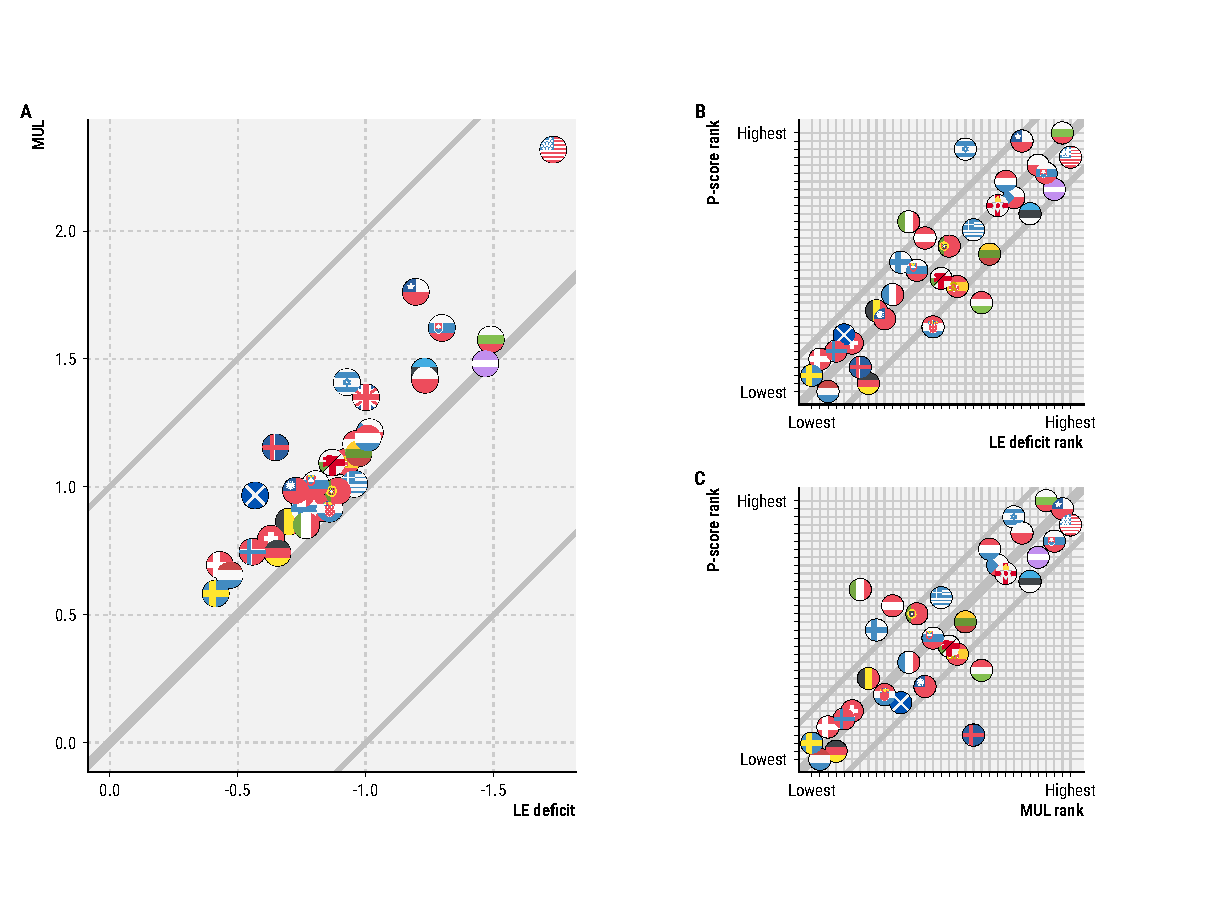
\includegraphics{92-excessmeasures20_24.pdf}
    \caption{Cross-country comparison of alternative excess mortality measures for the period 2020-2024. A) Life expectancy deficit vs. mean unfulfilled lifespan, B) Country ranking of life expectancy deficit vs. P-score, C) Country ranking of mean unfulfilled lifespan vs. P-score.}
    \label{fig:excessmeasures}
\end{figure}

\subsection{Sensitivity of results to choice of fitting period}

As a robustness check we re-calculated key results in our paper under a 10 year fitting period for the counterfactual life expectancy. Key results remain robust under either 10 or 20 years of fitting while the existence of significant life expectancy deficits in 2024 changes for some countries.

The cluster assignment under the hierarchical clustering algorithm is perfectly robust against changes in the fitting period with identical clusters identified under either analysis. Visually, the salient features of each cluster remain robust. A 10 year fitting period yields slightly lower life expectancy deficits 2020-24 compared to the longer fit (see Figures \ref{fig:deficit20y} and \ref{fig:deficit10y}).

\begin{figure}
    \centering
    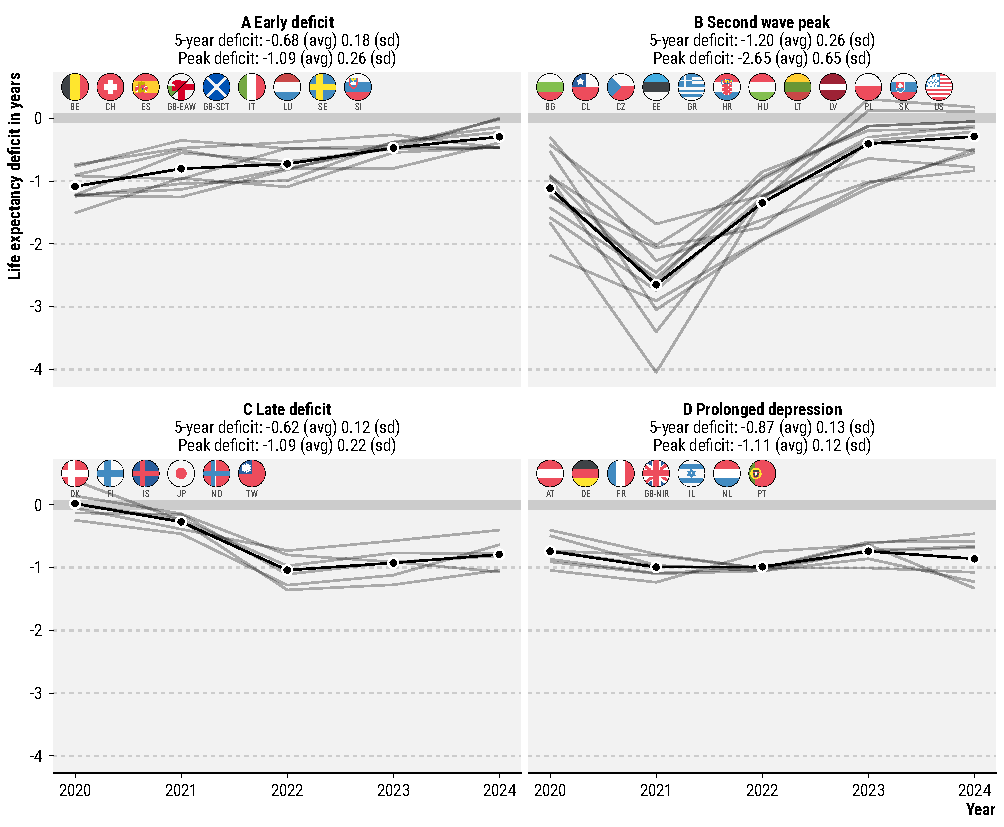
\includegraphics{60-e0deficittypology_20y_fitting_window.pdf}
    \caption{Deficit typology under 20 year Lee-Carter fitting period.}
    \label{fig:deficit20y}
\end{figure}


\begin{figure}
    \centering
    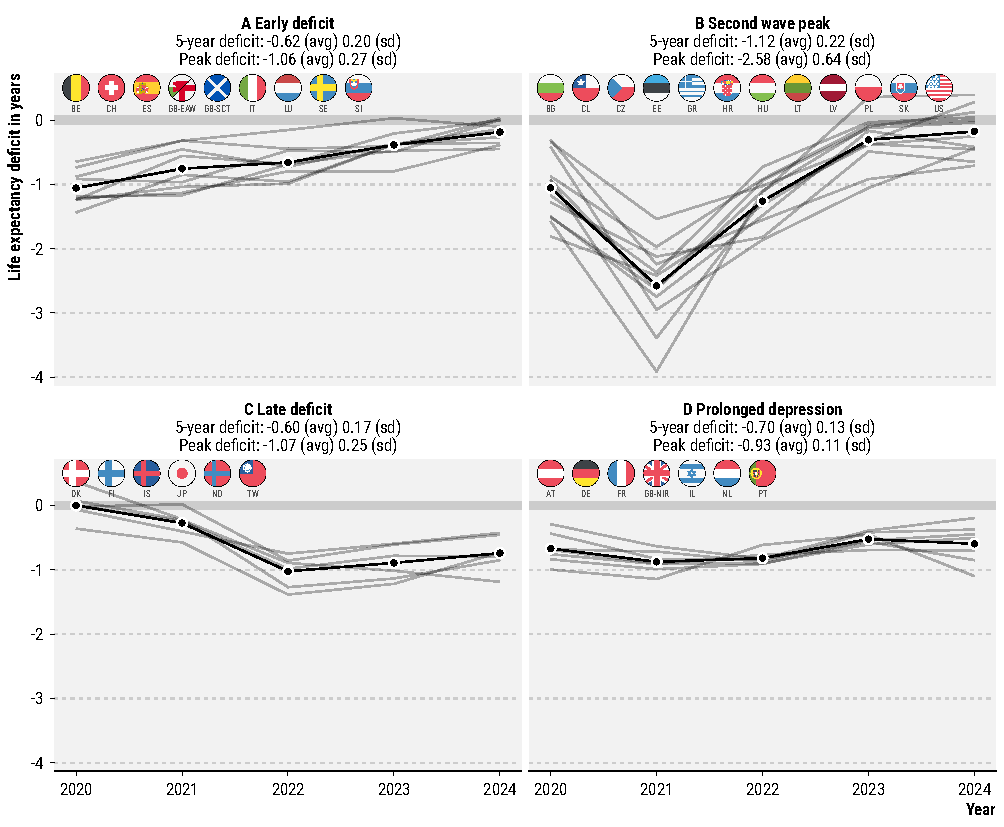
\includegraphics{60-e0deficittypology_10y_fitting_window.pdf}
    \caption{Deficit typology under 10 year Lee-Carter fitting period.}
    \label{fig:deficit10y}
\end{figure}

Under a 20 year fitting period we estimated 12 countries (AT, CL, DK, FI, GB-NIR, GR, IL, JP, NL, NO, TW, US) with a significant ($p<0.05$) life expectancy deficit in 2024 compared to 9 (CL, DK, FI, GB-NIR, IL, JP, NL, NO, TW) under a 10 year fit.

The US are uniquely sensitive to the choice of fitting period due to a period of life expectancy stagnation pre-2020. A 10 year fitting window continues the flat trajectory, leading to lower life expectancy deficits, whereas a 20 year fitting window extrapolates a longer term trend of slight life expectancy increase. As a result the finding that the US had the highest deficit overall is not robust (see Figures \ref{fig:annualdeficit20y} and \ref{fig:annualdeficit10y}).

\begin{figure}
    \centering
    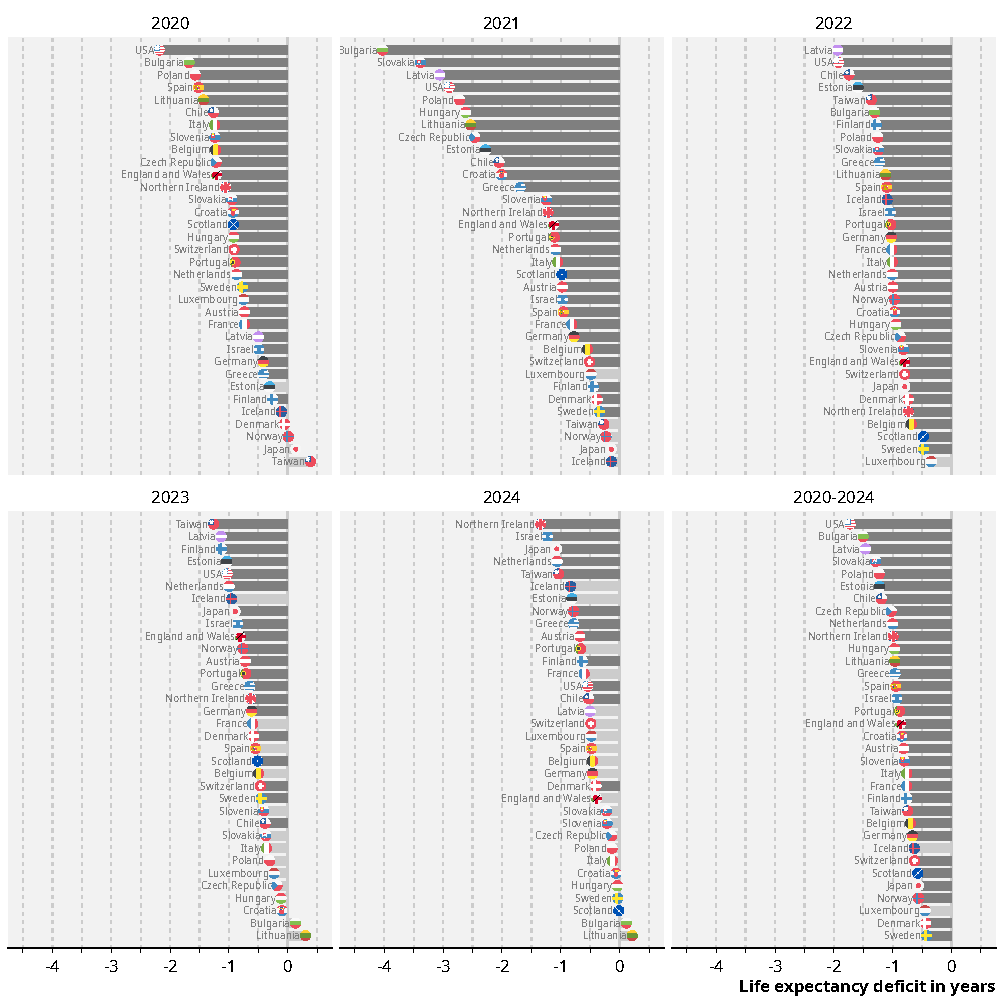
\includegraphics{61-e0deficitbyyear_total_20y_fitting_windows.pdf}
    \caption{Annual life expectancy deficits under 20 year Lee-Carter fitting period.}
    \label{fig:annualdeficit20y}
\end{figure}

\begin{figure}
    \centering
    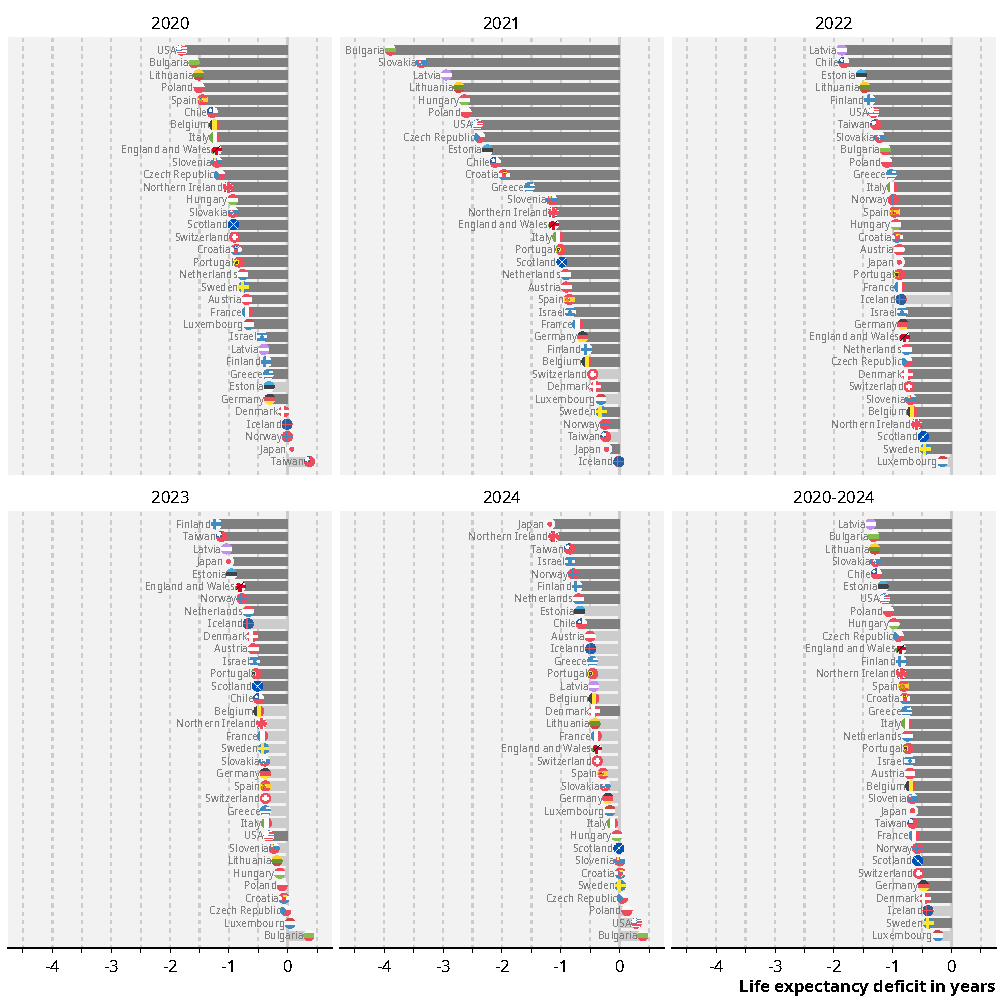
\includegraphics{61-e0deficitbyyear_total_10y_fitting_windows.pdf}
    \caption{Annual life expectancy deficits under 10 year Lee-Carter fitting period.}
    \label{fig:annualdeficit10y}
\end{figure}

\clearpage

\subsection{Sensitivity of results to choice of counterfactual}

The choice of model for producing the counterfactual life expectancy under continuation of pre-pandemic trends influences life expectancy deficit estimates. Here we compare our results under three different counterfactuals a) the Lee-Carter forecasts used in the main text, b) a direct extrapolation of 2019 life expectancy under continuation of the mean annual changes observed over 2000-2019 (LE random walk with drift), and c) a log-linear extrapolation of age specific death rates based on mean annual changes 2000-2019 (ASDR random walk with drift).

Figure \ref{fig:95-expected_by_model} displays the counterfactual life expectancy forecasts under different models. For the majority of locations the results are coherent. In countries where forecasts diverge noticeably, such as Estonia, Iceland, Israel, the Netherlands, Scotland, and the USA, the Lee-Carter model is always the least optimistic one, i.e. it produced lower counterfactual life expectancies compared with the alternative approaches. This tendency of the Lee-Carter model to be conservative in its forecasts makes our findings of life expectancy deficits conservative as well. The deficits we find tend to be even larger under alternative models.

\begin{figure}
    \centering
    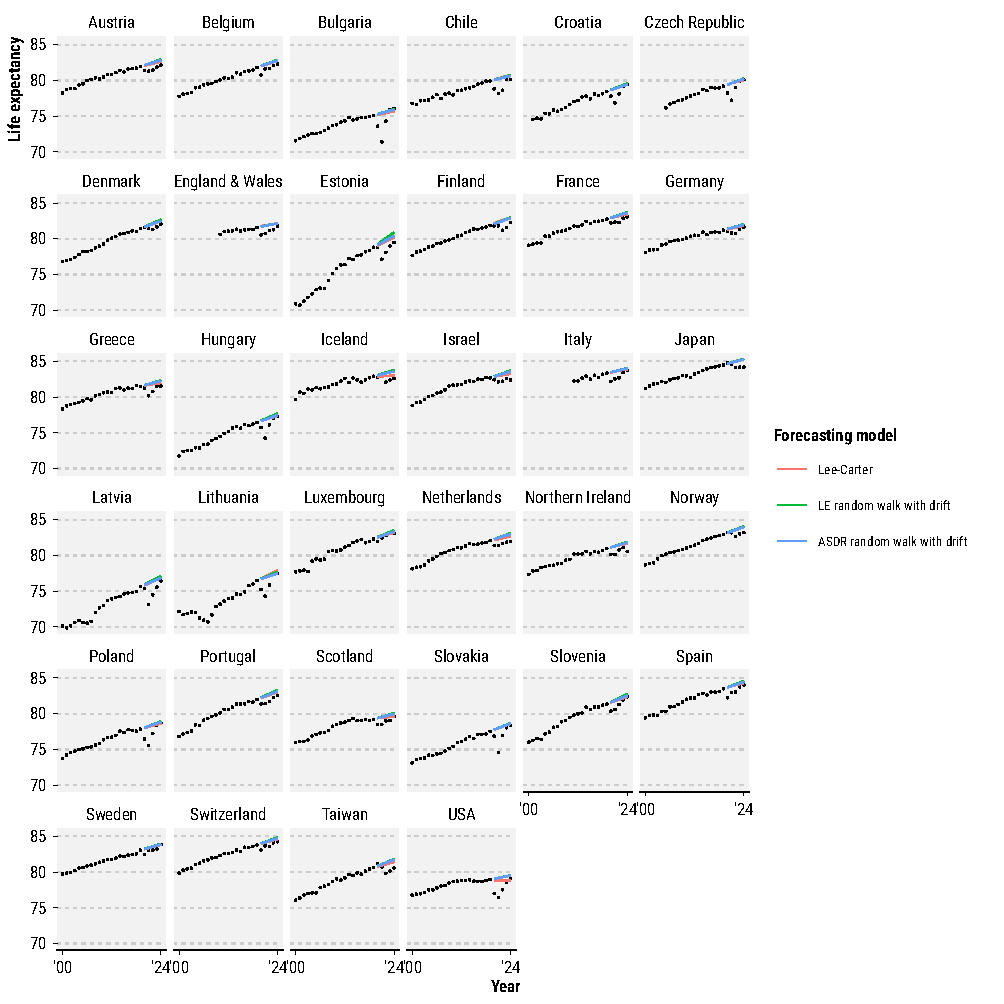
\includegraphics{95-expected_by_model.pdf}
    \caption{Comparison of life expectancy forecasts 2020-2024 under three different models.}
    \label{fig:95-expected_by_model}
\end{figure}

The country ranking in annual life expectancy deficits is somewhat sensitive to the choice of counterfactual model and becomes more sensitive over time as shown in Figure \ref{fig:95-deficit_rank_by_model}. However, almost all countries are within +/- 5 ranks of their Lee-Carter rank when comparing against the two alternative counterfactuals. Notable exceptions are the U.S. in 2023 and 2024 and Iceland in 2022. These changes in rank under different counterfactual life expectancy trajectories are however consistent with the prediction intervals given by the Lee-Carter method, which also derive from a set of simulated plausible counterfactuals. The prediction intervals around life expectancy deficits are wide enough to reliably identify the top, middle, and bottom groups in cross-country comparisons of life expectancy deficits, but do not allow for the robust identification of exact ranks.

\begin{figure}
    \centering
    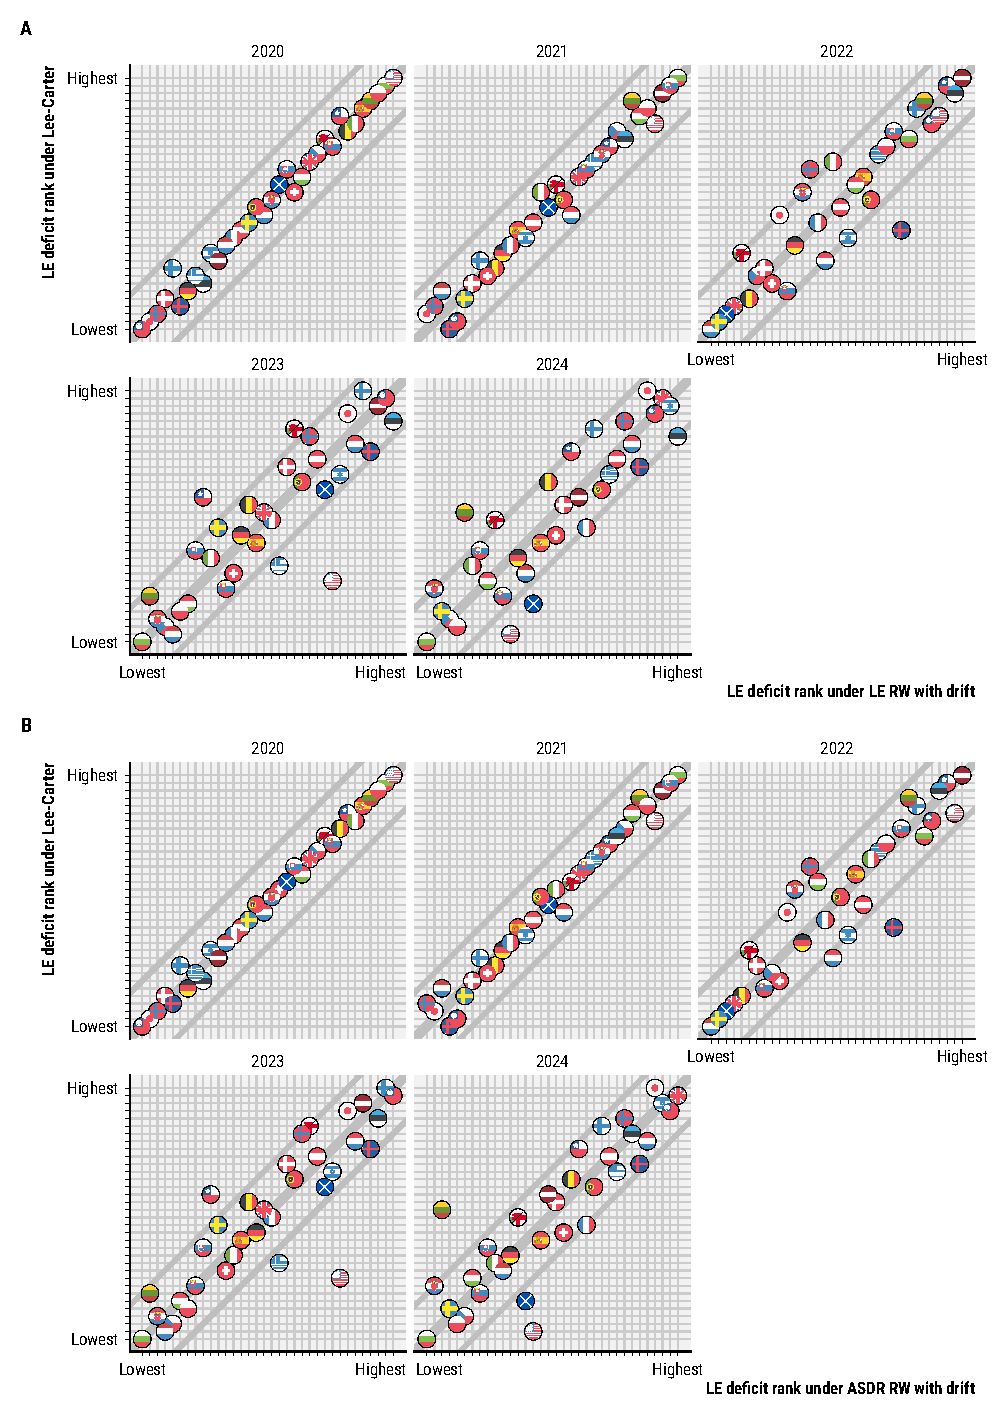
\includegraphics{95-deficit_rank_by_model.pdf}
    \caption{Country ranking of annual life expectancy deficits under different counterfactual models. Comparison of the Lee-Carter counterfactual with A) a direct extrapolation of life expectancy under continuation of average annual rate of increase over the time period 2000-2019, and B) a log-linear extrapolation of age specific death rates based on average changes over the time period 2000-2019.}
    \label{fig:95-deficit_rank_by_model}
\end{figure}

In Figure \ref{fig:95-deficit_cluster_by_model} we apply the same clustering as in the main text to life expectancy deficits under each counterfactual. Clearly the main cluster features reproduce almost perfectly across the different counterfactuals.

\begin{figure}
    \centering
    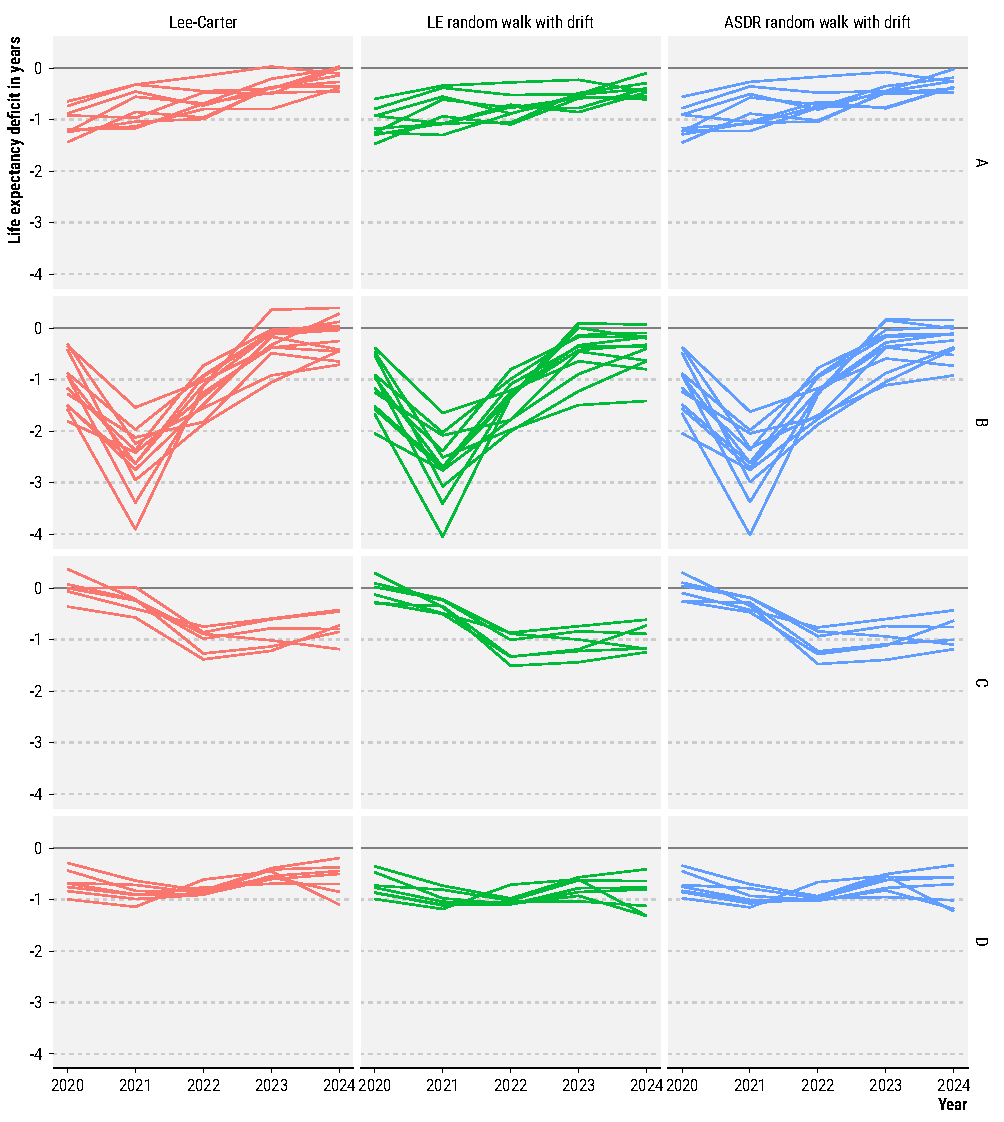
\includegraphics{95-deficit_cluster_by_model.pdf}
    \caption{Annual life expectancy deficits and clusters under different counterfactual models.}
    \label{fig:95-deficit_cluster_by_model}
\end{figure}

\clearpage

%--- Bibliography ------------------------------------------------------

\bibliography{refs.bib}

\clearpage

\end{document}
